\begin{center}
    \textbf{--------- Lezione 4 - 11 marzo 2021 ---------}
\end{center}
\begin{center}
    \textit{Augmented Reality (AR) is a live, direct or indirect, view of a physical, real-world environment whose elements are augmented by computer generated sensory input such as sound, video, graphic or GPS data}
\end{center}

AR è una vista live (in tempo reale) diretta (si può sovrapporre o sostituire al mondo reale) o indiretta (può aumentare una rappresentazione del mondo reale ad esempio una mappa) del mondo reale in cui andiamo a inserire delle informazioni, nell'ambiente, audio, video, grafica generate dal computer. 
\\ Abbiamo una sovrapposizione tra elementi del mondo reale e del mondo virtuale. 

L'AR indica quindi gli ambienti in cui si mescolano elementi del mondo reale e altri del mondo virtuale.
Quando si parla di sovrapporre elementi del mondo reale e del mondo virtuale, si parla di mixed reality. 
Si può dividere in due categorie:
\begin{itemize}
    \item augmented reality: elementi virtuali nel mondo reale
    \item augmented virtuality: elementi reali nel mondo virtuale
\end{itemize} 

Quando parliamo di un mondo AR dobbiamo dire cos'è del mondo reale e cosa del mondo virtuale.

Abbiamo diversi livelli di ambiente:
\begin{itemize}
    \item reality: solo l'ambiente reale
    \item mixed reality
    \item virtual reality: solo l'ambiente virtuale
\end{itemize}

AR esiste già dagli anni '40, non era digitale ma era ottenuta con tecniche analogiche.

Un esempio di applicazione di AR è anche la pubblicità proiettata nelle partite di NBA, la pubblicità non c'è veramente, è aggiunta virtualmente. 

L'AR non è solo visuale (anche se lo è per la maggior parte dei casi), ma può anche essere audio. 

Abbiamo 4 principali problemi:
\begin{itemize}
    \item Registration: ci permette di avere un modo di convertire le coordinate del mondo reale nelle coordinate dello schermo. Per fare ciò dobbiamo capire dove sta l'utente nel mondo reale
    \item Tracking: la registration ci permette di calcolare la conversione tra mondo reale e coordinate schermo in un dato istante, però dobbiamo tenere aggiornata questa cosa ad esempio quando muoviamo il device. L'aggiornamento si chiama tracking
    \item Display: gli oggetti virtuali nel mondo reale devono apparire realistici. Include sia operazioni di disegno, sia operazioni di comprensione dell'ambiente per far sì che quanto disegnato sia coerente con l’ambiente.
    Es: dove proiettare l'ombra dell'oggetto virtuale? Dobbiamo capire da dove arriva la luce. Abbiamo bisogno di tutta una serie di tecniche che ci permettano di capire dove devo collocare gli oggetti e dove li devo disegnare 
    \item Interaction: Vogliamo che gli oggetti virtuali appaiano come facenti parte dell'ambiente reale, come ad esempio un oggetto virtuale che deve apparire più grande se mi avvicino e più piccolo se mi allontano.
    Per questo dobbiamo comprendere com'è fatto l'ambiente, dov'è l'utente, come si sta muovendo e ho bisogno di poter interagire con gli oggetti reali e virtuali.Questo problema prende il nome di interaction
\end{itemize}



\section{Registration}
L'obiettivo è quello di creare un collegamento tra il mondo reale e il sistema di output. 
Bisogna capire come mappare le coordinate del mondo reale in coordinate dello schermo e viceversa. 
La registration ha molti aspetti in comune con il calcolo della posizione perché richiede di capire dove si trova l'utente rispetto ad un sistema di riferimento globale o locale.
Esistono 2 approcci alla registration:
\begin{itemize}
    \item basato su segnale radio
    \item basato su visione
\end{itemize}

\subsection{Registration con segnale radio}
Uno dei problemi principali è che è difficile calcolare la direzione dell'utente. 
Questa tecnica si può usare sia con una visione egocentrica (con la vista dell'utente) oppure per fare una visione allocentrica (vista dall'alto). 
Ad esempio un gioco in cui un utente, con una vista dall'alto, vede dei mostri virtuali muoversi su una mappa reale. L'utente stesso, perde se un mostro si avvicina a meno di 10 metri. Questo è un esempio di AR.  

\subsection{Registrazione visuale}
I sistemi basati su registrazione visuale ci permettono di registrarci rispetto ad un sistema locale. 
Non ci interessa la posizione rispetto al mondo ma rispetto a qualche sistema locale. 
Abbiamo tre soluzioni:
\begin{itemize}
    \item marcatori espliciti
    \item marcatori impliciti
    \item markerless
\end{itemize}

\subsubsection{Uso dei marcatori espliciti}
I marcatori sono sempre stati utilizzati fin dai primi sistemi di AR, per definire un sistema di riferimento, e permettono di calcolare l'orientamento con 6 gradi di libertà, con buona precisione, e l'omografia: un sistema per mappare le coordinate del mondo reale nelle coordinate schermo e viceversa. 

Gli oggetti visti dalla camera sono soggetti a trasformazione prospettica: le linee rette rimangono tali, ma angoli e distanze vengono alterati.

\begin{center}
    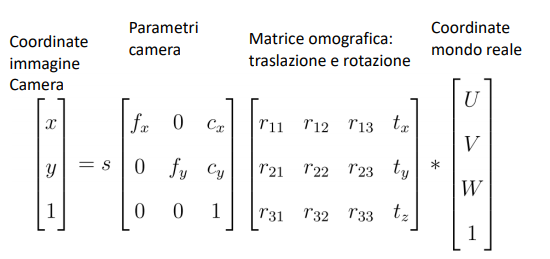
\includegraphics[width=.8\textwidth]{images/MobiDEV/3. augmented reality/matrice omografica.PNG}
\end{center}
Se riusciamo a calcolare questa matrice, possiamo convertire le coordinate. 

Dobbiamo creare un sistema di equazioni: 
\begin{itemize}
    \item alcuni parametri delle equazioni sono comuni (es: parametri della camera) 
    \item altri parametri sono in relazione nota tra di loro (es: se ho un marcatore, posso sapere la distanza tra i vertici). Serve conoscere almeno 4 coppie di punti (mondo reale e camera)
\end{itemize}
Se abbiamo almeno 4 coppie di punti nel mondo reale in relazione nota tra di loro e conosciamo i 4 corrispettivi punti nelle coordinate schermo, allora riusciamo a dare uno schema di equazioni che ci dà una soluzione approssimata a questo problema.

\vspace{10px}
\begin{minipage}{.5\textwidth}
   Una tecnica per il calcolo della posizione è l'utilizzo dei marcatori ARUCO.
   Hanno una forma quadrata, simile ai qr-code. Includono un disegno in bianco e nero, solitamente formato da pixel abbastanza grandi. I disegni non devono essere simmetrici perché vogliamo capire anche l'orientamento della camera. 
\end{minipage} 
\hfill
\begin{minipage}{.45\textwidth}
    \begin{center}
        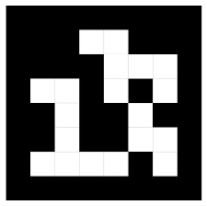
\includegraphics[width=.45\textwidth]{images/MobiDEV/3. augmented reality/aruco.PNG}
    \end{center}
\end{minipage}

\vspace{10px}
Come input abbiamo un'immagine A di un marcatore ARUCO, di cui è nota la dimensione, e un'immagine C presa dalla camera. Vogliamo calcolare se C contiene il codice ARUCO. Se non lo contiene non restituisco nulla, se lo contiene, restituisco la matrice omografica.
La procedura opera in questo modo:
\begin{enumerate}
    \item prende l'immagine dalla camera e la trasforma in bianco e nero. Prima l'immagine viene trasformata in scala di grigio, poi si usa un valore di soglia per trasformarla in bianco e nero
    \begin{center}
        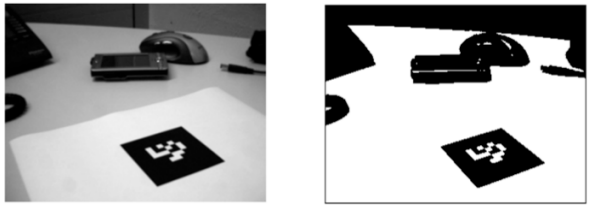
\includegraphics[width=.6\textwidth]{images/MobiDEV/3. augmented reality/1. aruco.PNG}
    \end{center}
    \item trova i quadrilateri. Si usano due tecniche: 
    \begin{itemize}
        \item Canny edge detection: permette di trovare i bordi, ovvero dove pixel bianchi e neri sono uno di fianco all'altro
        \item Hough line segment detection: permette di trovare i segmenti di retta
    \end{itemize}
    Quando ho i segmenti di retta posso trovare i quadrilateri (4 segmenti consecutivi che si vanno a chiudere).
    In visione prospettica vengono alterati gli angoli, ma le linee rette rimangono rette
    \begin{center}
        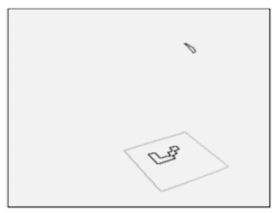
\includegraphics[width=.3\textwidth]{images/MobiDEV/3. augmented reality/2. aruco.PNG}
    \end{center}
    \item i quadrilateri trovati vengono processati uno ad uno e per ciascun quadrilatero Q:
    \begin{enumerate}[label*=\arabic*.]
        \item calcola l'omografia O assumendo che Q sia A (visto in prospettiva).
        Sappiamo qual è la posizione degli angoli nel mondo reale? 
        No, posizioniamo l'origine degli assi al centro dell'ARUCO. \\ Assumiamo che il quadrilatero Q sia effettivamente A, cioè che Q sia la visione prospettica di A. Prendiamo i 4 angoli del quadrilatero e calcoliamo l'omografia O usando le 4 equazioni degli angoli. 
        \\ Se non è l'ARUCO che mi interessa, calcolo la matrice omografica in modo sbagliato
        \item non so se quel quadrilatero sia l'ARUCO. Uso O per trasformare Q in Q', che è la vista di Q senza distorsione prospettica
        \begin{center}
            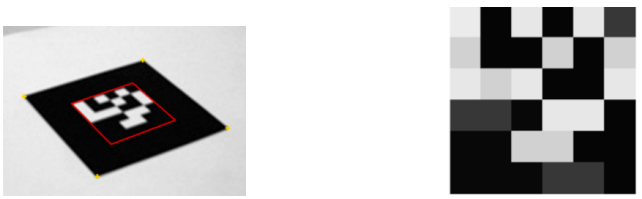
\includegraphics[width=.8\textwidth]{images/MobiDEV/3. augmented reality/3. aruco.PNG}
        \end{center}
    \end{enumerate}   
    \item se Q' corrisponde ad A, allora ritorno O. Se non corrisponde non torno nulla
\end{enumerate}

Fino ad ora non ho tenuto conto dell’orientamento del marcatore. Dovremmo calcolare ogni omografia per ciascuna possibile rotazione. 
Per ogni quadrilatero si possono calcolare 4 omografie (una per ogni possibile rotazione) oppure quando vado a confrontare Q’ con A, provo 4 volte, ruotando Q’ in tutte le possibili direzioni, poi se trovo la corrispondenza, adatto l’omografia.
\newpage